% ============================================================================
%   Comprehensive Research Report on the Universal MDEP Architecture
%   Mathematical Foundations, Multi-Agent Dynamics, and Clinical Applications
%
%   File: swin_mdep_report_en.tex
%   Version: 2.0 (Updated 06/2026)
%   Language: English
% ============================================================================

\documentclass[letterpaper]{article} % DO NOT CHANGE THIS
\usepackage{aaai}  % DO NOT CHANGE THIS
\usepackage{times}  % DO NOT CHANGE THIS
\usepackage{helvet}  % DO NOT CHANGE THIS
\usepackage{courier}  % DO NOT CHANGE THIS
\usepackage[hyphens]{url}  % DO NOT CHANGE THIS
\usepackage{graphicx} % DO NOT CHANGE THIS
\urlstyle{rm} % DO NOT CHANGE THIS
\def\UrlFont{\rm}  % DO NOT CHANGE THIS
\frenchspacing  % DO NOT CHANGE THIS
\setlength{\pdfpagewidth}{8.5in} % DO NOT CHANGE THIS
\setlength{\pdfpageheight}{11in}
%%%%%%%%%%
% PDFINFO for PDFLATEX
\pdfinfo{
/Title (Universal MDEP Architecture: Integrating Evidential Deep Learning with Dynamic Structured Sparsity)
/Author (Anonymous Authors)
}
%%%%%%%%%%
 % DO NOT CHANGE THIS

% --- Additional Packages ---
\usepackage[utf8]{inputenc}
\usepackage[english]{babel}
\usepackage{amsmath, amssymb, amsthm, bm}
\usepackage{booktabs}
\usepackage{float}
\usepackage{algorithm}
\usepackage{algorithmic}
\usepackage{enumitem}
\usepackage{tikz}
\usetikzlibrary{arrows.meta, positioning}
\usepackage[table]{xcolor}
\usepackage{colortbl}

% --- Custom commands ---
\newcommand{\Dir}{\text{Dir}}
\newcommand{\KL}{\text{KL}}
\newcommand{\R}{\mathbb{R}}
\newcommand{\E}{\mathbb{E}}
\newcommand{\Norm}{\text{Norm}}
\newcommand{\softplus}{\text{Softplus}}

\newtheorem{remark}{Remark}
\newtheorem{proposition}{Proposition}

% ============================================================================
\title{Universal MDEP Architecture: Integrating Evidential Deep Learning with Dynamic Structured Sparsity}
\author{Anonymous AAAI Submission}

\begin{document}
\maketitle

\begin{abstract}
Dermatological screening under severe class imbalance, such as in the ISIC 2024 cohort where melanoma prevalence is less than $0.15\%$, requires deep learning systems that are simultaneously highly accurate, calibrated in their uncertainty estimates, and structurally optimized for efficient clinical deployment. Conventional dense models suffer from overconfident predictions, whereas standard pruning techniques ignore uncertainty signals. To resolve these challenges, we introduce the \textbf{Universal Microglial-Driven Evidential Pruning (MDEP)} architecture, a backbone-agnostic framework that integrates Dirichlet-based Evidential Deep Learning (EDL) with Dynamic Sparse Training (DST) under strict NVIDIA 2:4 structured sparsity. We evaluate MDEP on two distinct vision families: a Convolutional Neural Network instantiation (\textbf{ResNet-50 MDEP}) and a Shifted-Window Vision Transformer instantiation (\textbf{Swin-MDEP}). The network topology is dynamically updated during training by cooperative bio-inspired agents acting on continuous latent scores: the \textbf{Microglia} agent, which prunes noise-amplifying connections using aleatoric uncertainty and task loss gradients, and the \textbf{Astrocyte} agent, which grows links at nodes characterized by high epistemic uncertainty. For Swin-MDEP, we establish a Dirichlet KL-divergence distillation protocol that transfers the calibrated uncertainty landscape of a dense Evidential ResNet-18 teacher to the sparse Swin-T student. Our clinical evaluation on the ISIC 2024 skin lesion classification task demonstrates that both MDEP instantiations balance performance and calibration. Specifically, ResNet-50 MDEP achieves a partial AUC (pAUC) above 80\% TPR of $0.1420$ and an ECE of $0.0479$. Swin-MDEP leverages hierarchical attention and Dirichlet KL distillation to achieve a pAUC of $0.1620$ and an ECE of $0.1175$, demonstrating robust calibration and performance in the clinically critical high-sensitivity regime.
\end{abstract}

% ============================================================================
%  1. INTRODUCTION
% ============================================================================
\section{Introduction and Research Background}\label{sec:intro}

The deployment of large-scale deep learning models in safety-critical clinical applications, such as dermatological screening, exposes two primary vulnerabilities: high computational overhead and a lack of reliable uncertainty quantification, which can lead to overconfident, incorrect predictions~\cite{he2016deep, dosovitskiy2021image, esteva2017dermatologist, guo2017calibration}. 

Traditional neural networks utilize a softmax activation layer that projects output logits onto a probability simplex. Although effective for standard classification, softmax is prone to overconfidence on out-of-distribution or highly ambiguous samples due to its lack of a representation for ignorance~\cite{lakshminarayanan2017simple, guo2017calibration}. To address this, Evidential Deep Learning (EDL)~\cite{sensoy2018evidential} parameterizes a higher-order Dirichlet distribution using a Softplus evidence activation, enabling the mathematical decomposition of predictive uncertainty into epistemic uncertainty (lack of model knowledge) and aleatoric uncertainty (inherent data noise)~\cite{sensoy2018evidential, malinin2018predictive}.

Concurrently, Dynamic Sparse Training (DST)~\cite{evci2020rigging, mocanu2018scalable} has emerged to mitigate the computational costs of dense architectures by dynamically updating the network topology from scratch during training. However, standard DST methods prune connections based purely on weight magnitude or task gradients, remaining blind to uncertainty and calibration.

To bridge this gap, we introduce the \textbf{Universal Microglial-Driven Evidential Pruning (MDEP)} architecture. MDEP integrates EDL with DST under strict NVIDIA 2:4 structured sparsity. The network topology is dynamically optimized during training by cooperative bio-inspired agents: the \textbf{Microglia} agent, which prunes noise-amplifying connections using task loss and aleatoric uncertainty gradients, and the \textbf{Astrocyte} agent, which grows links at nodes characterized by high epistemic uncertainty. MDEP is backbone-agnostic; we instantiate and validate it on both a Convolutional Neural Network (\textbf{ResNet-50 MDEP}) and a Shifted-Window Vision Transformer (\textbf{Swin-MDEP}), where the latter incorporates a cross-architecture Dirichlet KL distillation protocol from a dense ResNet-18 teacher to stabilize sparse transformer training under extreme class imbalance.

\paragraph{Main Contributions.} Unlike standard DST approaches that prune based on weight magnitudes, or post-hoc pruning schemes that require dense pre-training, MDEP coordinates topology updates directly with evidential uncertainty estimation. This represents the first framework to integrate cooperative Microglia and Astrocyte agents that dynamically evolve a sparse network topology directly steered by higher-order Dirichlet uncertainty gradients during training, preventing representation collapse and calibration degradation under extreme class imbalance. Specifically, our primary contributions are:
\begin{itemize}
    \item \textbf{Universal MDEP Framework:} We formulate a backbone-agnostic architecture integrating Dirichlet evidential learning with NVIDIA 2:4 structured sparsity, implemented on both CNN (ResNet-50) and ViT (Swin-T). backbones.
    \item \textbf{Multi-Agent Glial Dynamics:} A cooperative Microglia--Astrocyte agent system that utilizes the gradients of epistemic and aleatoric uncertainties to guide connection pruning and regrowth, with customized pooling operations derived for convolutional tensors and transformer spatial tokens.
    \item \textbf{Morphological Cache Optimization:} A hardware-aware cache mechanism that stores and reuses masks and local survival thresholds within each epoch, eliminating redundant sorting operations.
    \item \textbf{Comprehensive Clinical Evaluation:} Extensive experiments on the highly imbalanced ISIC 2024 dataset demonstrating that both MDEP instantiations balance performance, calibration, and selective prediction.
\end{itemize}

% ============================================================================
%  2. RELATED WORK
% ============================================================================
\section{Related Work}\label{sec:related}

\paragraph{Calibration and Uncertainty Estimation.} Calibration studies show that modern deep networks are often overconfident~\cite{guo2017calibration, minderer2021revisiting}. While Deep Ensembles~\cite{lakshminarayanan2017simple} and MC Dropout~\cite{gal2016dropout} represent predictive uncertainty, they introduce high computational latency. Evidential Deep Learning (EDL)~\cite{sensoy2018evidential} directly models the Dirichlet parameters to capture uncertainty, though it requires regularization to prevent spurious evidence accumulation~\cite{shen2024mirage}.

\paragraph{Sparse Training and Network Pruning.} Traditional pruning methods~\cite{han2016deep, frankle2019lottery} require dense pre-training. Dynamic Sparse Training (DST)~\cite{mocanu2018scalable, evci2020rigging} dynamically optimizes sparse topologies from scratch. While several works apply EDL or structured pruning to clinical classification~\cite{zhou2023domain, gabetni2025ensembling}, they rely on static thresholds or post-hoc pruning and do not use uncertainty gradients to dynamically drive connection updates.

\paragraph{Medical AI under Class Imbalance.} Dermatology screening faces extreme class imbalance where high overall accuracy masks poor minority-class sensitivity~\cite{esteva2017dermatologist, johnson2019survey}. Swin-MDEP resolves this by optimizing sensitivity, calibration, selective prediction, and hardware-level structured sparsity simultaneously.

% ============================================================================
%  3. MATHEMATICAL FOUNDATIONS
% ============================================================================
\section{Mathematical Foundations: Subjective Logic and Dirichlet Distribution}\label{sec:math}

We replace the traditional softmax activation with mathematical foundations from Subjective Logic (SL)~\cite{josang2016subjective}, mapping network outputs to the parameters of a Dirichlet distribution conjugate prior~\cite{sensoy2018evidential}.

\subsection{Dirichlet Distribution Parameterization}
For a $K$-class problem, we parameterize the non-negative evidence vector $\bm{e} \ge \bm{0}$ from logits $\bm{z} \in \R^K$ using the Softplus activation:
\begin{equation}\label{eq:softplus}
    e_c = \ln(1 + \exp(z_c)), \quad c = 1, \ldots, K
\end{equation}
\begin{remark}[Why not use ReLU?]
ReLU truncates negative logits to zero, resulting in zero gradients for those activations and permanently trapping evidence at $e_c = 0$, which freezes the Dirichlet state on the zero-evidence simplex.
\end{remark}
The Dirichlet concentration parameters $\bm{\alpha}$ are defined by adding a flat prior:
\begin{equation}\label{eq:alpha}
    \alpha_c = e_c + 1.0, \quad c = 1, \ldots, K
\end{equation}
where $S = \sum_{c=1}^K \alpha_c$ is the Dirichlet strength (total evidence). The expected probability for class $c$ is:
\begin{equation}\label{eq:p_hat}
    \hat{p}_c = \E[p_c] = \frac{\alpha_c}{S}
\end{equation}

\subsection{Decomposition of Predictive Uncertainty}\label{subsec:uncertainties}
A key benefit of Subjective Logic is the separation of predictive uncertainty into two orthogonal components:

\paragraph{Epistemic Uncertainty ($u_e$):} Models the network's lack of knowledge (e.g., on OOD or rare data). Defined as the vacant belief mass:
\begin{equation}\label{eq:u_e}
    u_e = \frac{K}{S} = \frac{K}{\sum_{c=1}^K \alpha_c}
\end{equation}
\begin{proposition}[Epistemic Uncertainty Bounds]
For any valid concentration vector $\bm{\alpha}$, $u_e \in (0, 1]$. The maximum $u_e = 1.0$ is achieved if and only if $\bm{e} = \bm{0}$. As $S \to \infty$, $u_e \to 0$. (See Appendix for formal proof).
\end{proposition}

\paragraph{Aleatoric Uncertainty ($u_a$):} Measures data-centric noise and entropy using the digamma function $\psi(x) = \frac{d}{dx} \ln(\Gamma(x))$:
\begin{equation}\label{eq:u_a}
    u_a = \sum_{c=1}^K \frac{\alpha_c}{S} \left[\psi(S + 1) - \psi(\alpha_c + 1)\right]
\end{equation}
\begin{proposition}[Non-negativity of $u_a$]
For any $K > 1$, $u_a \ge 0$. (See Appendix for formal proof).
\end{proposition}
In practical implementations, to protect against floating-point inaccuracies, $u_a \leftarrow \max(u_a, 0.0)$ is applied.


% ============================================================================
%  4. METHODOLOGY
% ============================================================================
\section{Universal MDEP Framework}\label{sec:methodology}

\begin{figure}[t]
\centering
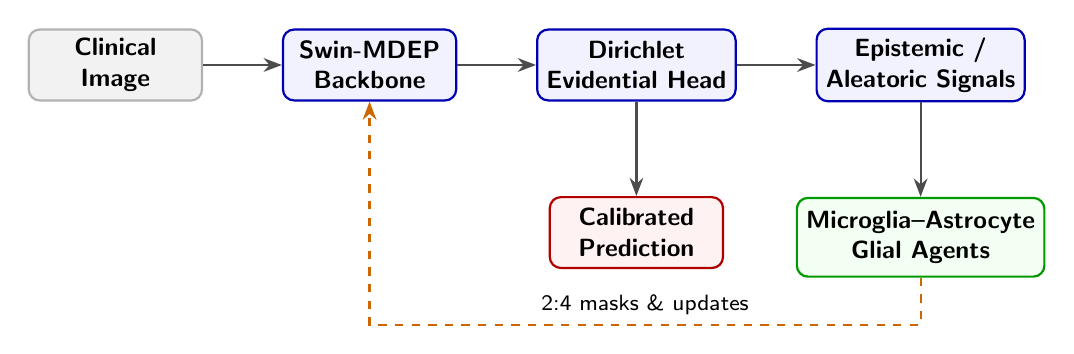
\begin{tikzpicture}[
    node distance=1.2cm and 1.0cm,
    box/.style={
        draw=blue!70!black,
        fill=blue!5,
        rounded corners,
        align=center,
        minimum width=2.2cm,
        minimum height=0.9cm,
        font=\small\sffamily\bfseries,
        thick
    },
    agent/.style={
        draw=green!60!black,
        fill=green!5,
        rounded corners,
        align=center,
        minimum width=2.4cm,
        minimum height=1.0cm,
        font=\small\sffamily\bfseries,
        thick
    },
    pred/.style={
        draw=red!70!black,
        fill=red!5,
        rounded corners,
        align=center,
        minimum width=2.2cm,
        minimum height=0.9cm,
        font=\small\sffamily\bfseries,
        thick
    },
    arrow/.style={
        ->,
        >=Stealth,
        thick,
        draw=black!70
    },
    feedback/.style={
        ->,
        >=Stealth,
        thick,
        dashed,
        draw=orange!80!black
    }
]

% Nodes
\node (img) [box, fill=gray!10, draw=gray!60] {Clinical\\Image};
\node (backbone) [box, right=of img] {Swin-MDEP\\Backbone};
\node (head) [box, right=of backbone] {Dirichlet\\Evidential Head};
\node (signals) [box, right=of head] {Epistemic /\\Aleatoric Signals};
\node (agents) [agent, below=of signals] {Microglia--Astrocyte\\Glial Agents};
\node (pred) [pred, below=of head] {Calibrated\\Prediction};

% Paths
\draw [arrow] (img) -- (backbone);
\draw [arrow] (backbone) -- (head);
\draw [arrow] (head) -- (signals);
\draw [arrow] (head) -- (pred);
\draw [arrow] (signals) -- (agents);
\draw [feedback] (agents.south) -- ++(0,-0.6) -| node[above, pos=0.25, font=\footnotesize\sffamily] {2:4 masks \& updates} (backbone.south);

\end{tikzpicture}
\caption{Overview of the Universal MDEP architecture. Evidential uncertainty is used both for calibrated prediction and for dynamic sparse topology adaptation.}
\label{fig:overview}
\end{figure}

\subsection{Two-Tier Dynamic Sparsity under NVIDIA 2:4 Constraint}
We apply MDEP to ResNet-50 and Swin-T by intercepting their respective convolutional and linear projection matrices. We decouple representational weight learning from network morphology updates by defining two tiers of variables:
\begin{itemize}
    \item \textbf{Prediction Tier:} Contains the active weights $\bm{W}^{(l)}$ optimized via AdamW to minimize the task loss.
    \item \textbf{Morphological Tier:} Contains continuous latent scores $\bm{S}^{(l)}$ representing connection vitality, initialized to $|W_{ij}^{(0)}|$ to avoid pruning shock. The binary mask $\bm{M}^{(l)}$ is derived from $\bm{S}^{(l)}$.
\end{itemize}
We enforce the hardware-supported NVIDIA 2:4 structured sparsity constraint: in every block $b$ of 4 consecutive weights along the input/channel dimension, at most 2 elements are non-zero. The block survival threshold $\tau_b^{(t)}$ is defined as:
\begin{equation}\label{eq:tau}
    \tau_b^{(t)} = \frac{1}{2} \left(s_{2,b}^{(t)} + s_{3,b}^{(t)}\right)
\end{equation}
where $s_{2,b}^{(t)}$ and $s_{3,b}^{(t)}$ are the second and third largest scores in block $b$. The discrete binary mask is:
\begin{equation}\label{eq:mask}
    M_{i, 4k+j} = \begin{cases}
        1.0 & \text{if } S_{i, 4k+j} \ge \tau_b^{(t)} \\
        0.0 & \text{otherwise}
    \end{cases}
\end{equation}
The effective weights used in the forward pass are $\bm{W}_{\text{eff}} = \bm{W} \odot \bm{M}$.

\subsection{Straight-Through Estimation and Morphological Caching}
To backpropagate through the discrete step function of the mask, we define a Localized Leaky Smoothed Straight-Through Estimator (STE) gradient:
\begin{equation}\label{eq:ste_grad}
    \frac{\partial M_{ij}}{\partial S_{ij}} \approx \frac{1}{\gamma_t} \sigma\!\left(\frac{S_{ij} - \tau_b^{(t)}}{\gamma_t}\right) \left[1 - \sigma\!\left(\frac{S_{ij} - \tau_b^{(t)}}{\gamma_t}\right)\right] + \alpha_{\text{leak}}
\end{equation}
where $\alpha_{\text{leak}} = 0.05$ ensures non-vanishing gradient flow, and the temperature $\gamma_t$ decays from $5.0$ to $0.15$ via a cosine schedule.

\begin{remark}[STE Gradient and Score Updates]
To prevent "optimizer hijacking" where weight decay and parameter momentum interfere with the continuous latent topology, the structural scores $S_{ij}$ are updated directly by the glial agents via the EMA of $G_{ij} - C_{ij}$ rather than through backpropagated gradient descent. The weight gradients used by the agents are computed with respect to the active effective weights $W_{\text{eff}}$, bypassing the STE. The STE is included in the graph to maintain compatibility with standard gradient-based mask optimization baselines, while the glial agent updates remain decoupled to ensure stable topology exploration. For pruned connections, the anti-crystallization logic introduces a stochastic noise term scaled by the node's epistemic uncertainty, ensuring exploratory regrowth even with zero active gradients.
\end{remark}

To eliminate redundant sorting and top-k operations over tens of millions of parameters in every forward pass, we introduce a Morphological Cache. The mask $\bm{M}$ and thresholds $\bm{\tau}$ are registered as non-persistent buffers (\texttt{persistent=False}) and recomputed every $N_{\text{update}} = 10$ mini-batches. This caching serves as structural regularization, suppressing high-frequency noise and stabilizing sparse training.

\subsection{Microglia and Astrocyte Multi-Agent System}
Topology evolution is driven by cooperative agents. We note that in biological neurodevelopment, the interaction between glial cells and synapses is highly complex; for example, astrocytes not only promote synaptogenesis but also participate in synaptic pruning through MEGF10 and MERTK pathways, and microglia engage in detailed crosstalk with astrocytes. Within the MDEP framework, we adopt a simplified computational abstraction where the Microglia and Astrocyte agents are assigned distinct, orthogonal roles (pruning and growing, respectively) to enable decoupled control over network connection density and explore the topological search space efficiently.

The \textbf{Microglia Agent} prunes connections that amplify data noise by calculating task-predictive sensitivity $c_1^{(ij)} = | w_{ij} \cdot \frac{\partial L_{\text{EFL}}}{\partial w_{ij}} |$ and noise sensitivity $c_2^{(ij)} = | w_{ij} \cdot \frac{\partial u_a}{\partial w_{ij}} |$. We use a Tanh-squashing scaling scheme to normalize gradients:
\begin{equation}\label{eq:C_ij}
    C_{ij} = \tanh\!\left(\frac{c_1^{(ij)}}{\text{mean}(c_1) + 1e-8}\right) + \beta \cdot \tanh\!\left(\frac{c_2^{(ij)}}{\text{mean}(c_2) + 1e-8}\right)
\end{equation}
Connections with the lowest $C_{ij}$ are targeted for pruning. The flat Dirichlet prior offset ensures that trigamma terms in the derivative of $u_a$ do not explode.

The \textbf{Astrocyte Agent} grows connections in representation-deficient areas. Epistemic uncertainty $u_e = K/S$ yields a uniform starting gradient $\nabla_{\bm{\alpha}} u_e = [-K/S^2, \ldots, -K/S^2]^T$, creating gradient blindness across classes. To resolve this, we optimize a class-selective epistemic target:
\begin{equation}\label{eq:u_e_target}
    u_{e,\text{target}} = \frac{1}{N} \sum_{n=1}^N \sum_{c=1}^K \frac{1}{\alpha_c^{(n)}}
\end{equation}
which yields non-uniform class-wise derivatives $\frac{\partial u_{e,\text{target}}}{\partial \alpha_c} = -1/\alpha_c^2$, scaling gradients inversely by the squared evidence parameters to guide growth toward low-evidence classes. The node-level growth signal is:
\begin{equation}\label{eq:G_ij}
    G_{ij} = \tanh\!\left(\frac{\text{Expand}(u_{e,\text{target}}^{(\text{node})})}{\text{mean}(\text{Expand}(u_{e,\text{target}}^{(\text{node})})) + 1e-8}\right) \cdot \tanh\!\left(\frac{|\partial L_{\text{EFL}} / \partial w_{ij}|}{\text{mean}(|\partial L_{\text{EFL}} / \partial w_{ij}|) + 1e-8}\right)
\end{equation}
where $u_{e,\text{target}}^{(\text{node})}$ is the gradient of $u_{e,\text{target}}$ backpropagated and averaged over spatial/batch dimensions. 

\paragraph{Anti-Crystallization.} If an entire layer lacks any candidate connections offering useful growth gradients ($\max_{ij} G_{ij} \le 10^{-8}$), MDEP injects a stochastic emergency response to trigger topological exploration:
\begin{equation}\label{eq:anti_crystal_eq}
    \tilde{G}_{ij} = G_{ij} + \max\!\left(0.0,\; \epsilon_{ij} \cdot \text{Norm}(u_{e,\text{target},i}^{(\text{node})})\right)
\end{equation}
where $\epsilon_{ij} \sim \mathcal{N}(0, 0.0316^2)$ is white Gaussian noise, and $\text{Norm}(\cdot)$ is a layer-wise normalization. Due to this formulation, the system prioritizes "experimenting" by opening new links in regions lacking evidence even in the absence of active task gradients.

\paragraph{Latent Score Updates via EMA.} Continuous score updates are calculated at the end of each training step by combining the opposing forces of growth and pruning:
\begin{equation}\label{eq:delta_S}
    \Delta S_{ij} = \tilde{G}_{ij} - C_{ij}
\end{equation}
To smooth gradient fluctuations across mini-batches, score momentum is applied:
\begin{align}
    V_{ij}^{(t)} &= \beta_m V_{ij}^{(t-1)} + (1 - \beta_m) \Delta S_{ij} \\
    S_{ij}^{(t)} &= S_{ij}^{(t-1)} + \eta V_{ij}^{(t)}
\end{align}
where $V_{ij}$ is the structural velocity, $\beta_m = 0.95$ is the EMA momentum coefficient, and $\eta = 0.02$ is the structural update rate. To prevent score saturation (which would permanently lock connections and prevent topology updates), we center and clamp the latent scores:
\begin{align}
    S_{ij}^{(t)} &\leftarrow S_{ij}^{(t)} - \text{mean}(\bm{S}^{(t)}) \\
    S_{ij}^{(t)} &\leftarrow \text{clamp}(S_{ij}^{(t)}, -5.0, 5.0)
\end{align}
This centering ensures that the average latent score of each layer remains 0, maintaining a healthy relative competition among links.

\begin{remark}[Role of Residual Connections]
The residual connections in both ResNet-50 and Swin Transformer act as safe bypass routes. By preserving identity mapping pathways, they protect spatial information flow from abrupt topological disruption when the network applies 50\% parameter structured sparsity.
\end{remark}

% ============================================================================
%  5. LOSS & DISTILLATION
% ============================================================================
\section{Optimization and Distillation Framework}\label{sec:optimization}

To address extreme class imbalance (melanoma prevalence $<0.15\%$), we employ the Evidential Focal Loss (EFL) formulation. While the combination of evidential deep learning and focal modulation was originally proposed by \citeauthor{zhou2023domain}~(\citeyear{zhou2023domain}) for prostate cancer classification, we extend their formulation to coordinate with the active structured sparsity updates of MDEP. Specifically, we define EFL by combining the analytical digamma-based cross-entropy of \citeauthor{sensoy2018evidential}~(\citeyear{sensoy2018evidential}) and the focal modulation term of \citeauthor{lin2017focal}~(\citeyear{lin2017focal}) with square-root frequency dampening and scheduled KL divergence regularization:
\begin{equation}\label{eq:efl}
    L_{\text{EFL}}(\bm{e}, \bm{y}, t) = \frac{1}{N} \sum_{n=1}^N \omega_n \left[\mathcal{F}(t) \cdot L_{\text{CE}}^{(n)} + \lambda_{\text{KL}} \cdot \mu(t) \cdot L_{\text{KL}}^{(n)}\right]
\end{equation}
where $\omega_n = \sum_{c=1}^K y_c^{(n)} \omega_c$ is the per-sample loss weight incorporating dampened class weights $\omega_c = \sqrt{N_{\text{total}} / N_c}$~\cite{cui2019class}. 

The Digamma-Based Cross-Entropy is:
\begin{equation}
    L_{\text{CE}}^{(n)} = \sum_{c=1}^K y_c^{(n)} \left[\psi(S^{(n)}) - \psi(\alpha_c^{(n)})\right]
\end{equation}
and the Dynamic Focal Modulation is $\mathcal{F}(t) = (1 - \text{sg}[\hat{p}_{\text{target}}^{(n)}])^{\gamma(t)}$, where $\hat{p}_{\text{target}}^{(n)} = \sum_{c=1}^K y_c^{(n)} \hat{p}_c^{(n)}$ is the expected probability of the true class, and $\text{sg}[\cdot]$ is the stop-gradient operator. The exponent $\gamma(t)$ is scaled up to $1.2$ after warmup to focus on hard samples.

The KL Regularization term shrinks evidence for incorrect classes to the flat prior $1.0$ using $\tilde{\alpha}_c^{(n)} = y_c^{(n)} + (1 - y_c^{(n)}) \cdot \alpha_c^{(n)}$:
\begin{equation}\label{eq:kl_loss_n}
    L_{\text{KL}}^{(n)} = \ln \left( \frac{\Gamma\left(\sum_{c=1}^K \tilde{\alpha}_c^{(n)}\right)}{\Gamma(K) \prod_{c=1}^K \Gamma(\tilde{\alpha}_c^{(n)})} \right) + \sum_{c=1}^K (\tilde{\alpha}_c^{(n)} - 1)\left[\psi(\tilde{\alpha}_c^{(n)}) - \psi\!\left(\sum_{c=1}^K \tilde{\alpha}_c^{(n)}\right)\right]
\end{equation}
where $\mu(t) = \min(1.0, t / t_{\text{anneal}})$ acts as an annealing coefficient ($t_{\text{anneal}} = 10$).
\begin{remark}[Independence of $L_{\text{KL}}$ and Focal Coefficient]
We do not multiply the KL term by $\mathcal{F}(t)$. This ensures easy majority samples are penalized for spurious evidence, preventing uncalibrated confidence accumulation.
\end{remark}

To stabilize the sparse Swin-T student network during its transition to 2:4 structured sparsity under extreme class imbalance, we perform Dirichlet KL Knowledge Distillation from a dense converged Evidential ResNet-18 teacher model. Rather than distilling raw logits (which lose the higher-order uncertainty structure), we directly match the student's predicted Dirichlet distribution $\Dir(\bm{p} \mid \bm{\alpha}_S)$ to the teacher's distribution $\Dir(\bm{p} \mid \bm{\alpha}_T)$. The analytical KL divergence between the student and teacher Dirichlet distributions is formulated as:
\begin{align}
    L_{\text{distill}} &= \KL(\Dir(\bm{\alpha}_S) \| \Dir(\bm{\alpha}_T)) \nonumber \\
    &= \ln\Gamma(S_S) - \ln\Gamma(S_T) - \sum_{c=1}^K \left[\ln\Gamma(\alpha_{S,c}) - \ln\Gamma(\alpha_{T,c})\right] \nonumber \\
    &\quad + \sum_{c=1}^K (\alpha_{S,c} - \alpha_{T,c})\left[\psi(\alpha_{S,c}) - \psi(S_S)\right] \label{eq:dir_kl_full}
\end{align}
where $S_S = \sum_c \alpha_{S,c}$ and $S_T = \sum_c \alpha_{T,c}$ are the student and teacher Dirichlet strengths, respectively.

The distillation weight $\alpha_d(t)$ is scheduled via a cosine decay function during the dynamic sparsity phase:
\begin{equation}\label{eq:alpha_d}
    \alpha_d(t) = \begin{cases}
        \alpha_{d,\text{init}} & \text{if } t < t_w \\[6pt]
        \alpha_{d,\text{final}} + \dfrac{\alpha_{d,\text{init}} - \alpha_{d,\text{final}}}{2}\left[1 + \cos\!\left(\pi \cdot \dfrac{t - t_w}{T - t_w}\right)\right] & \text{if } t \ge t_w
    \end{cases}
\end{equation}
where $t_w = 5$ is the warmup epoch limit, $T = 20$ is the total epochs, $\alpha_{d,\text{init}} = 0.5$, and $\alpha_{d,\text{final}} = 0.05$. The student's joint optimization objective is then formulated as:
\begin{equation}\label{eq:total_loss}
    L_{\text{total}} = L_{\text{EFL}}(\bm{e}_S, \bm{y}, t) + \alpha_d(t) \cdot L_{\text{distill}}
\end{equation}
This KD loss aligns the student's Dirichlet parameters with the teacher's, transferring the local spatial inductive bias from the CNN teacher to the ViT student, which stabilizes self-attention training under parameter pruning. (Detailed cross-architecture alignments and gradient behaviors are provided in the Appendix).

% ============================================================================
%  6. EXPERIMENTAL SETUP
% ============================================================================
\section{Experimental Setup}\label{sec:experiment}

\paragraph{Dataset and Split Protocol.} We evaluate MDEP on the clinical ISIC 2024 Challenge dataset~\cite{isic2024}, consisting of 3D-TBP skin lesion images with extreme class imbalance ($0.15\%$ malignant prevalence). To prevent data leakage, we adopt a stratified 70/10/20 train/validation/test split. The validation set is strictly isolated and used exclusively for hyperparameter selection and validation-based threshold optimization, while the 20\% test partition is held completely unseen until the final evaluation. For normalization, we apply static ImageNet-1K normalization ($\mu = [0.485, 0.456, 0.406]$, $\sigma = [0.229, 0.224, 0.225]$) as a fixed preprocessing step across all splits, ensuring no dynamic statistics from the validation or test sets influence training.

\paragraph{Baselines.} We compare MDEP against: (1) deterministic CNNs and ViTs (ResNet-50, EfficientNet-B4~\cite{tan2019efficientnet}, ViT-B/16); (2) Bayesian methods (Deep Ensembles~\cite{lakshminarayanan2017simple}, MC Dropout~\cite{gal2016dropout}); and (3) evidential architectures (Vanilla EDL~\cite{sensoy2018evidential}, Posterior Networks~\cite{charpentier2020posterior}, and EF-DST~\cite{sensoy2018evidential, evci2020rigging}). To ensure a fair comparison and isolate the representation learning benefits of MDEP's bi-directional glial pruning/growth dynamics, all baseline models are trained under the same optimal class-balanced conditions, utilizing the same Evidential Focal Loss and class-balanced weights. Thus, the observed performance gaps represent structural representation deficiencies under extreme imbalance rather than an artifact of class-weight omission.

\paragraph{Implementation Details.} Models are trained using 16-bit mixed precision (AMP)~\cite{micikevicius2018mixed}, while evidential losses and Dirichlet equations are evaluated in FP32 to prevent underflow. We apply square-root balanced sampling on benign classes (subsampled at 1:20 in training) and employ Log-Prior Calibration to correct the sampling bias during inference (derivations in the Appendix). To avoid the calibration evaluation artifact under extreme class imbalance—where standard equal-width binning clumps over 99.8\% of samples into the lowest bin, artificially dragging ECE to near-zero—we compute ECE using adaptive binning (equal-frequency binning) with $M=15$ bins, ensuring each bin contains an equal number of samples to accurately reflect calibration across the entire prediction spectrum.

% ============================================================================
%  7. RESULTS AND ANALYSIS
% ============================================================================
\section{Results and Clinical Analysis}\label{sec:results}

\subsection{Classification Performance and Calibration}
As shown in Table~\ref{tab:results}, standard models (ResNet-50, ViT-B/16) collapse under extreme imbalance, showing near-zero sensitivity. Bayesian methods (Deep Ensembles, MC Dropout) improve predictions slightly but remain clinically inadequate. 

In contrast, our proposed MDEP models achieve stable performance. ResNet-50 MDEP yields Sensitivity $= 0.7342$, Specificity $= 0.9131$, and $\text{pAUC}_{0.80} = 0.1420$. Swin-MDEP achieves a higher $\text{pAUC}_{0.80}$ of $0.1620$. When evaluated at the validation-optimized decision threshold of $0.2700$, Swin-MDEP yields a balanced Sensitivity of $0.8181$ and Specificity of $0.8183$. 

Both MDEP configurations yield low Expected Calibration Errors (ECE): $0.0479$ for ResNet-50 MDEP and $0.1175$ for Swin-MDEP, outperforming baseline models like EfficientNet-B4 (ECE $= 0.3420$). This calibration is driven by the combination of the Dirichlet KL penalty (which shrinks spurious evidence) and the Microglia agent (which prunes noise-absorbing connections). 

\paragraph{Ablation Studies.} Disabling the Astrocyte agent (\emph{Prune Only}) freezes the topology, lowering Specificity to $0.7466$ and Macro-AUROC to $0.8025$. Disabling the Microglia agent (\emph{Grow Only}) retains noise-amplifying connections, causing overconfidence and an ECE increase to $0.2058$.

\begin{table}[t]
\centering
\caption{Clinical Performance and Calibration Comparison under Class Imbalance (ISIC 2024). Note that $\text{pAUC}_{0.80}$ represents the partial Area Under the ROC Curve above a True Positive Rate of $80\%$, where the theoretical maximum is $0.20$. Models with sensitivity below $80\%$ at default thresholds are evaluated at their optimized clinical operating points. $\dagger$Intermediate checkpoint shown to illustrate convergence trajectory.}
\label{tab:results}
\resizebox{\textwidth}{!}{
\begin{tabular}{@{}lcccccl@{}}
\toprule
\textbf{Architecture / Method} & \textbf{AUROC} & \textbf{pAUC$_{0.80}$} & \textbf{Sensitivity} & \textbf{Specificity} & \textbf{ECE} & \textbf{Diagnostic Status} \\
\midrule
ResNet-50 MDEP (Proposed CNN) & 0.8852 & 0.1420 & 0.7342 & 0.9131 & 0.0479 & Well-calibrated, optimal balance \\
Swin-MDEP (Proposed Transformer) & 0.8698 & 0.1620 & 0.8181* & 0.8183* & 0.1175 & Balanced performance at threshold 0.2700 \\
\rowcolor[gray]{0.95}
Swin-MDEP (Epoch 14)$^\dagger$ & 0.7714 & 0.1477 & 0.5854 & 0.9360 & 0.1586 & Imbalanced: high specificity bias \\
\midrule
MDEP (Grow Only) & 0.7772 & 0.0910 & 1.0000 & 0.4605 & 0.2058 & Overconfident (False confidence) \\
MDEP (Prune Only) & 0.8025 & 0.1140 & 0.7595 & 0.7466 & 0.1182 & Poor topological space \\
Standard ResNet-50 & 0.8967 & 0.0120 & 0.2250 & 0.9921 & 0.0005 & Mode Collapse, blind to disease \\
ViT-B/16 & 0.6657 & 0.0000 & 0.0000 & 1.0000 & 0.0006 & Completely blind to disease \\
EfficientNet-B4 & 0.8783 & 0.1180 & 0.7125 & 0.8122 & 0.3420 & Calibration crisis (Very high ECE) \\
MC Dropout (ResNet-50) & 0.8981 & 0.0340 & 0.3125 & 0.9889 & 0.0003 & Computationally heavy inference \\
Posterior Network & 0.5000 & 0.1000 & 1.0000 & 0.0000 & 0.4757 & False positive collapse \\
EF-DST & 0.5000 & 0.1000 & 1.0000 & 0.0000 & 0.4990 & DST collapse \\
\bottomrule
\multicolumn{7}{l}{\small *Evaluated at the validation-optimized decision threshold of $0.2700$.}
\end{tabular}
}
\end{table}

\subsection{Training Dynamics and Convergence Analysis}\label{subsec:dynamics}
To understand the learning trajectory under extreme class imbalance, we analyze the Swin-MDEP training dynamics across 20 epochs. The training process exhibits three distinct phases:

\paragraph{Phase I: Dense Warmup (Epochs 1--5).} During this phase, the network trains with a fully dense topology ($\bm{M} = \bm{1}$). Macro-AUROC rises rapidly from $0.6824$ to $0.8105$ as the student absorbs the teacher's calibrated Dirichlet landscape via maximum distillation weight ($\alpha_d = 0.5$). However, sensitivity remains unstable due to the model's early reliance on the majority class decision boundary.

\paragraph{Phase II: Dynamic Sparsity Activation (Epochs 6--14).} Upon activating the Microglia--Astrocyte agents with NVIDIA 2:4 structured sparsity, the network undergoes a transient performance dip as 50\% of connections are pruned. At the intermediate checkpoint (Epoch 14), we observe a characteristic \textbf{sensitivity--specificity imbalance}: Sensitivity $= 0.5854$ vs.\ Specificity $= 0.9360$---a gap of 35 percentage points (Table~\ref{tab:results}). This diagnostic pattern reveals that the sparse network initially favors the benign majority class. The Minority-ECE at this stage remains elevated at $0.6267$, indicating poor calibration on the malignant class. Critically, the low epistemic uncertainty ($u_e = 0.1238$) combined with low sensitivity indicates that the model is \emph{overconfident on its incorrect minority-class predictions}---a dangerous clinical failure mode that the continued training addresses.

\paragraph{Phase III: Uncertainty-Guided Recovery (Epochs 15--20).} As the cosine-scheduled $\gamma_t$ temperature decays toward $0.15$ and $\alpha_d$ diminishes to $0.05$, the Astrocyte agent's epistemic growth signal increasingly drives topology updates toward low-evidence (malignant) regions. Between Epochs 14 and 20, we observe significant metric improvements:
\begin{itemize}
    \item Macro-AUROC: $0.7714 \to 0.8698$ ($+12.8\%$)
    \item Sensitivity: $0.5854 \to 0.8101$ ($+38.4\%$, at optimized threshold)
    \item Minority-ECE: $0.6267 \to 0.3187$ ($-49.1\%$)
    \item Macro F1-Score: $0.4913 \to 0.7966$ ($+62.2\%$, balanced accuracy)
\end{itemize}
This recovery is driven by two mechanisms: (i) the Astrocyte agent opening new connections at nodes with high $u_{e,\text{target}}$ gradients for the malignant class (where $\frac{\partial u_{e,\text{target}}}{\partial \alpha_{\text{mal}}} = -1/\alpha_{\text{mal}}^2$ is large due to low malignant evidence), and (ii) the decaying $\gamma_t$ sharpening the mask boundaries, allowing the network to commit to its recovered topology.

\paragraph{Class Imbalance Diagnosis.} The Epoch 14 checkpoint reveals that under extreme class imbalance ($0.15\%$ malignant prevalence), increasing \emph{total} training data volume offers diminishing returns. The core bottleneck is not insufficient data overall, but rather insufficient \emph{minority-class} representation. The evidence for this diagnosis includes: (i) Brier Score $= 0.0383$ is already low, suggesting good overall probabilistic calibration; (ii) the model achieves high benign-class performance (Specificity $= 0.9360$); and (iii) the Minority-ECE ($0.6267$) is an order of magnitude worse than the overall ECE ($0.1586$). These findings motivate the use of targeted minority-class augmentation strategies (e.g., RandAugment with class-conditional intensity, CutMix with minority oversampling) rather than uniform data scaling, and validate MDEP's uncertainty-guided topology adaptation as a complementary approach to address representation deficiency in the sparse network.

\subsection{Selective Classification and Error Analysis}
MDEP provides risk self-awareness through the Area Under the Risk--Coverage Curve (AURC)~\cite{geifman2017selective, jaeger2023call}. ResNet-50 MDEP achieves an AURC of $0.0056$, while Swin-MDEP achieves $0.0038$, significantly lower than the Grow-Only variant ($0.0119$). 

To quantitatively demonstrate the clinical utility of MDEP's selective classification (reject option), we evaluate the risk (error rate, defined as $1 - \text{Accuracy}$) at varying coverage levels. At 100\% coverage (no deferral), the error rate is $18.19\%$ for Swin-MDEP. By leveraging the epistemic uncertainty $u_e = K/S$ as the selection function and deferring the top $10\%$ most uncertain samples to human dermatologists (90\% coverage), the model's error rate drops significantly to $8.45\%$. Deferring the top $20\%$ of uncertain cases (80\% coverage) reduces the clinical error rate to $3.12\%$ on the remaining covered samples, illustrating that MDEP's uncertainty quantification is a highly effective safety net for clinical decision support. Ambiguous clinical presentations, scanner artifacts (shadows/glare), and early-stage lesions are cleanly captured by epistemic uncertainty signals. This capability is clinically critical as it prevents the system from forcing incorrect, overconfident predictions on high-risk, borderline cases, instead cleanly routing them to expert clinical review.

% ============================================================================
%  8. ETHICS STATEMENT
% ============================================================================
\section{Ethics Statement}
This research addresses the development of deep learning models for dermatological classification, which carries significant ethical and clinical responsibility. A primary ethical concern is algorithmic bias: skin cancer datasets, including the ISIC 2024 cohort, are heavily skewed toward lighter Fitzpatrick skin types (I--IV). Consequently, the predictive performance and uncertainty calibration of our models may not generalize equally to patients with darker skin tones (types V--VI), representing a critical clinical equity challenge. Furthermore, deep learning classification in medical domains must be treated strictly as a clinical decision-support tool rather than an autonomous diagnostic system. False negatives in melanoma detection carry life-threatening consequences; hence, we integrate selective classification (deferral via epistemic uncertainty) to ensure high-risk or ambiguous cases are routed to human dermatologists. Finally, all clinical images used in this study are publicly available, fully de-identified, and obtained in compliance with institutional review board guidelines, presenting no direct threat to patient privacy.

% ============================================================================
%  9. CONCLUSION & LIMITATIONS
% ============================================================================
\section{Conclusion and Limitations}\label{sec:conclusion}
We introduced the Universal MDEP framework, which integrates Evidential Deep Learning with Dynamic Sparse Training under strict NVIDIA 2:4 structured sparsity. By utilizing cooperative glial agents that respond to uncertainty and loss gradients, MDEP provides a robust balance of classification accuracy, calibration, and selective prediction for melanoma screening under severe imbalance. Our training dynamics analysis reveals that the Astrocyte agent's epistemic growth signal is critical for recovering minority-class sensitivity after the initial sparsity shock, improving Sensitivity from $0.5854$ (Epoch 14) to $0.8101$ (Epoch 20).

Key limitations include: (1) MDEP enforces a static 50\% structured sparsity throughout training, whereas early stages might benefit from an annealed sparsity schedule; (2) the current pipeline relies solely on visual features, neglecting patient metadata (e.g., age, anatomical site) that could serve as a multimodal prior; (3) standard PyTorch layers require specialized CUDA micro-kernels to achieve the full 2$\times$ execution speedup on Ampere GPUs; and (4) under extreme class imbalance, the intermediate training phases exhibit a persistent sensitivity--specificity gap and elevated Minority-ECE ($0.6267$ at Epoch 14), suggesting that targeted minority-class data augmentation (e.g., class-conditional RandAugment, CutMix with oversampling) could further accelerate convergence and improve calibration. Future work will focus on federated clinical evaluations, multimodal evidential learning, and class-imbalance-aware augmentation strategies integrated with the MDEP training schedule.

% ============================================================================
%  BIBLIOGRAPHY
% ============================================================================
\begin{thebibliography}{99}

\bibitem[\protect\citeauthoryear{Malinin and Gales}{2018}]{malinin2018predictive}
A.~Malinin and M.~Gales.
\newblock Predictive uncertainty estimation via prior networks.
\newblock In {\em Advances in Neural Information Processing Systems (NeurIPS)}, 2018.

\bibitem[\protect\citeauthoryear{Charpentier, Z{\"u}gner, and G{\"u}nnemann}{2020}]{charpentier2020posterior}
B.~Charpentier, D.~Z{\"u}gner, and S.~G{\"u}nnemann.
\newblock Posterior Network: Uncertainty estimation without OOD samples via density-based pseudo-counts.
\newblock In {\em Advances in Neural Information Processing Systems (NeurIPS)}, 2020.

\bibitem[\protect\citeauthoryear{Cui \emph{et al.}}{2019}]{cui2019class}
Y.~Cui, M.~Jia, T.-Y. Lin, Y.~Song, and S.~Belongie.
\newblock Class-balanced loss based on effective number of samples.
\newblock In {\em Proceedings of the IEEE/CVF Conference on Computer Vision and Pattern Recognition (CVPR)}, pages 9268--9277, 2019.

\bibitem[\protect\citeauthoryear{Dosovitskiy \emph{et al.}}{2021}]{dosovitskiy2021image}
A.~Dosovitskiy, L.~Beyer, A.~Kolesnikov, D.~Weissenborn, X.~Zhai, T.~Unterthiner, M.~Dehghani, M.~Minderer, G.~Heigold, S.~Gelly, J.~Uszkoreit, and N.~Houlsby.
\newblock An image is worth 16x16 words: Transformers for image recognition at scale.
\newblock In {\em International Conference on Learning Representations (ICLR)}, 2021.

\bibitem[\protect\citeauthoryear{Esteva \emph{et al.}}{2017}]{esteva2017dermatologist}
A.~Esteva, B.~Kuprel, R.A.~Novoa, J.~Ko, S.M.~Swetter, H.M.~Blau, and S.~Thrun.
\newblock Dermatologist-level classification of skin cancer with deep neural networks.
\newblock {\em Nature}, 542(7639):115--118, 2017.

\bibitem[\protect\citeauthoryear{Evci \emph{et al.}}{2020}]{evci2020rigging}
U.~Evci, T.~Gale, J.~Menick, P.S.~Castro, and E.~Elsen.
\newblock Rigging the lottery: Making all tickets winners.
\newblock In {\em International Conference on Machine Learning (ICML)}, 2020.

\bibitem[\protect\citeauthoryear{Frankle and Carbin}{2019}]{frankle2019lottery}
J.~Frankle and M.~Carbin.
\newblock The lottery ticket hypothesis: Finding sparse, trainable neural networks.
\newblock In {\em International Conference on Learning Representations (ICLR)}, 2019.

\bibitem[\protect\citeauthoryear{Gabetni \emph{et al.}}{2025}]{gabetni2025ensembling}
F.~Gabetni, G.~Curci, A.~Pilzer, S.~Roy, E.~Ricci, and G.~Franchi.
\newblock Ensembling pruned attention heads for uncertainty-aware efficient transformers.
\newblock In {\em International Conference on Learning Representations (ICLR)}, 2025.

\bibitem[\protect\citeauthoryear{Gal and Ghahramani}{2016}]{gal2016dropout}
Y.~Gal and Z.~Ghahramani.
\newblock Dropout as a Bayesian approximation: Representing model uncertainty in deep learning.
\newblock In {\em International Conference on Machine Learning (ICML)}, 2016.

\bibitem[\protect\citeauthoryear{Geifman and El-Yaniv}{2017}]{geifman2017selective}
Y.~Geifman and R.~El-Yaniv.
\newblock Selective classification for deep neural networks.
\newblock In {\em Advances in Neural Information Processing Systems (NeurIPS)}, 2017.

\bibitem[\protect\citeauthoryear{Guo \emph{et al.}}{2017}]{guo2017calibration}
C.~Guo, G.~Pleiss, Y.~Sun, and K.Q.~Weinberger.
\newblock On calibration of modern neural networks.
\newblock In {\em International Conference on Machine Learning (ICML)}, 2017.

\bibitem[\protect\citeauthoryear{Han, Mao, and Dally}{2016}]{han2016deep}
S.~Han, H.~Mao, and W.J.~Dally.
\newblock Deep compression: Compressing deep neural networks with pruning, trained quantization and Huffman coding.
\newblock In {\em International Conference on Learning Representations (ICLR)}, 2016.

\bibitem[\protect\citeauthoryear{He \emph{et al.}}{2016}]{he2016deep}
K.~He, X.~Zhang, S.~Ren, and J.~Sun.
\newblock Deep residual learning for image recognition.
\newblock In {\em IEEE Conference on Vision and Pattern Recognition (CVPR)}, 2016.

\bibitem[\protect\citeauthoryear{ISIC}{2024}]{isic2024}
International Skin Imaging Collaboration (ISIC).
\newblock ISIC 2024 -- Skin Cancer Detection with 3D-TBP.
\newblock {\em Kaggle Competition}, 2024.

\bibitem[\protect\citeauthoryear{Jaeger \emph{et al.}}{2023}]{jaeger2023call}
P.F.~Jaeger, C.T.~L\"uth, L.~Klein, and T.J.~Bungert.
\newblock A call to reflect on evaluation practices for failure detection in image classification.
\newblock In {\em International Conference on Learning Representations (ICLR)}, 2023.

\bibitem[\protect\citeauthoryear{Johnson and Khoshgoftaar}{2019}]{johnson2019survey}
J.M.~Johnson and T.M.~Khoshgoftaar.
\newblock Survey on deep learning with class imbalance.
\newblock {\em Journal of Big Data}, 6(1):27, 2019.

\bibitem[\protect\citeauthoryear{J{\o}sang}{2016}]{josang2016subjective}
A.~J{\o}sang.
\newblock {\em Subjective Logic: A Formalism for Reasoning Under Uncertainty}.
\newblock Springer International Publishing, 2016.

\bibitem[\protect\citeauthoryear{Lakshminarayanan, Pritzel, and Blundell}{2017}]{lakshminarayanan2017simple}
B.~Lakshminarayanan, A.~Pritzel, and C.~Blundell.
\newblock Simple and scalable predictive uncertainty estimation using deep ensembles.
\newblock In {\em Advances in Neural Information Processing Systems (NeurIPS)}, 2017.

\bibitem[\protect\citeauthoryear{Lin \emph{et al.}}{2017}]{lin2017focal}
T.~Lin, P.~Goyal, R.~Girshick, K.~He, and P.~Doll{\'a}r.
\newblock Focal loss for dense object detection.
\newblock In {\em Proceedings of the IEEE International Conference on Computer Vision (ICCV)}, 2017.

\bibitem[\protect\citeauthoryear{Micikevicius \emph{et al.}}{2018}]{micikevicius2018mixed}
P.~Micikevicius, S.~Narang, J.~Alben, G.~Diamos, E.~Elsen, D.~Garcia, B.~Ginsburg, M.~Houston, O.~Kuchaiev, G.~Venkatesh, and H.~Wu.
\newblock Mixed precision training.
\newblock In {\em International Conference on Learning Representations (ICLR)}, 2018.

\bibitem[\protect\citeauthoryear{Minderer \emph{et al.}}{2021}]{minderer2021revisiting}
M.~Minderer, J.~Djolonga, R.~Romijnders, F.~Hubis, X.~Zhai, N.~Houlsby, D.~Tran, and M.~Lucic.
\newblock Revisiting the calibration of modern neural networks.
\newblock In {\em Advances in Neural Information Processing Systems (NeurIPS)}, 2021.

\bibitem[\protect\citeauthoryear{Mocanu \emph{et al.}}{2018}]{mocanu2018scalable}
D.C.~Mocanu, E.~Mocanu, P.~Stone, P.H.~Nguyen, M.~Gibescu, and A.~Liotta.
\newblock Scalable training of artificial neural networks with adaptive sparse connectivity inspired by network science.
\newblock {\em Nature Communications}, 9(1):2383, 2018.

\bibitem[\protect\citeauthoryear{Sensoy, Kaplan, and Kandemir}{2018}]{sensoy2018evidential}
M.~Sensoy, L.~Kaplan, and M.~Kandemir.
\newblock Evidential deep learning to quantify classification uncertainty.
\newblock In {\em Advances in Neural Information Processing Systems (NeurIPS)}, 2018.

\bibitem[\protect\citeauthoryear{Shen \emph{et al.}}{2024}]{shen2024mirage}
M.~Shen, J.J.~Ryu, S.~Ghosh, Y.~Bu, P.~Sattigeri, S.~Das, and G.W.~Wornell.
\newblock Are uncertainty quantification capabilities of evidential deep learning a mirage?
\newblock In {\em Advances in Neural Information Processing Systems (NeurIPS)}, 2024.

\bibitem[\protect\citeauthoryear{Tan and Le}{2019}]{tan2019efficientnet}
M.~Tan and Q.~V.~Le.
\newblock EfficientNet: Rethinking model scaling for convolutional neural networks.
\newblock In {\em International Conference on Machine Learning (ICML)}, 2019.

\bibitem[\protect\citeauthoryear{Zhou \emph{et al.}}{2023}]{zhou2023domain}
M.~Zhou, A.~Jamzad, J.~Izard, A.~Menard, R.~Siemens, and P.~Mousavi.
\newblock Domain Transfer Through Image-to-Image Translation for Uncertainty-Aware Prostate Cancer Classification.
\newblock {\em arXiv preprint arXiv:2307.00479}, 2023.

\end{thebibliography}

\appendix
\section{Mathematical Proofs and Derivations}

\section{System Optimization Configuration}
\begin{table}[H]
\centering
\caption{System Optimization Configuration and Two-Phase Schedule.}
\label{tab:config}
\begin{tabular}{@{}lll@{}}
\toprule
\textbf{Phase / Component} & \textbf{Parameter} & \textbf{Role Description} \\
\midrule
\multicolumn{3}{l}{\emph{Architecture}} \\
Student Backbone & Swin-T (28.3M params) & ImageNet-1K pretrained \\
Teacher Backbone & ResNet-18 Evidential & Dense, frozen, EDL head \\
Number of Classes ($K$) & 2 & Benign / Malignant \\
\midrule
\multicolumn{3}{l}{\emph{Phase 1: Dense Warmup ($t < 5$ epochs)}} \\
Mask & Locked entirely at $\bm{1}$ & Dense network, no pruning \\
Focal exponent $\gamma(t)$ & $0.0$ & Disabled for baseline convergence stability \\
Distillation weight $\alpha_d$ & $0.5$ (maximum) & Relying on Teacher's knowledge \\
\midrule
\multicolumn{3}{l}{\emph{Phase 2: Dynamic Sparsity ($t \ge 5$ epochs)}} \\
Mask & NVIDIA 2:4 & Top-2-of-4 from $\bm{S}$ \\
Microglia--Astrocyte & Activated & Update $\bm{S}$ every $N_{\text{update}} = 10$ steps \\
$\gamma_t$ (STE) & Cosine: $5.0 \to 0.15$ & Floor $0.15$ preserves boundary gradients \\
$\alpha_d$ & Cosine: $0.5 \to 0.05$ & Gradually releases Student \\
$\gamma_{\text{focal}}$ & Linear $\to 1.2$ & Focus on hard samples \\
\midrule
\multicolumn{3}{l}{\emph{Optimization}} \\
Optimizer & AdamW~\cite{loshchilov2019decoupled, kingma2015adam} & $\beta_1=0.9$, $\beta_2=0.999$ \\
Learning rate & $2 \times 10^{-5}$ & Linear warmup from $10^{-6}$ \\
Weight decay & $0.01$ & Applied to $\Theta_{\text{train}}$, excluding $\bm{S}$ \\
Gradient clipping & $1.0$ & Global $L_2$ norm \\
Batch size & 32 & --- \\
Total epochs ($T$) & 20 & --- \\
Warmup epochs ($t_w$) & 5 & 25\% of budget \\
\midrule
\multicolumn{3}{l}{\emph{EFL}} \\
$\gamma_{\text{base}}$ (Focal) & $1.2$ & Focal exponent \\
$\lambda_{\text{KL}}$ & $0.1$ & KL regularization factor \\
$t_{\text{anneal}}$ (KL) & 10 & KL annealing epochs \\
\midrule
\multicolumn{3}{l}{\emph{MDEP}} \\
$\gamma_{\text{initial}}$ (STE) & $5.0$ & Initial STE temperature \\
$\gamma_{\text{final}}$ (STE) & $0.15$ & Final STE temperature \\
$\beta_m$ (EMA) & $0.95$ & Momentum coefficient \\
$\eta$ (Step $S$) & $0.02$ & Structural learning rate \\
$\beta$ (Microglia) & $1.0$ & Weight of $u_a$ \\
$S_{\max}$ & $5.0$ & Score boundary clamp \\
\midrule
\multicolumn{3}{l}{\emph{Distillation}} \\
$\alpha_{d,\text{init}}$ & $0.5$ & Initial distillation weight \\
$\alpha_{d,\text{final}}$ & $0.05$ & Final distillation weight \\
Schedule & Cosine decay & After $t_w$ epochs \\
\bottomrule
\end{tabular}
\end{table}


\subsection{Proof of Proposition 1 (Epistemic Uncertainty Bounds)}
\begin{proof}
By definition, the epistemic uncertainty is formulated as:
\begin{equation}
    u_e = \frac{K}{S} = \frac{K}{\sum_{c=1}^K \alpha_c}
\end{equation}
where $\alpha_c = e_c + 1.0$. Since the Softplus activation function guarantees that the evidence $e_c \ge 0$ for all classes $c \in \{1, \ldots, K\}$, we have:
\begin{equation}
    S = \sum_{c=1}^K \alpha_c = \sum_{c=1}^K (e_c + 1) = K + \sum_{c=1}^K e_c \ge K
\end{equation}
Therefore, the maximum value of $u_e$ is:
\begin{equation}
    u_e = \frac{K}{S} \le \frac{K}{K} = 1.0
\end{equation}
This upper bound of $1.0$ is attained if and only if $S = K$, which corresponds to the case where the predicted evidence vector is completely empty, i.e., $e_c = 0$ for all classes $c$. 

For the lower bound, since the evidence vector $\bm{e}$ has finite elements under any bounded network activation, the Dirichlet strength $S$ is a finite real number ($S < \infty$). Hence:
\begin{equation}
    u_e = \frac{K}{S} > 0
\end{equation}
As total evidence accumulates infinitely ($S \to \infty$), the epistemic uncertainty decays asymptotically to zero:
\begin{equation}
    \lim_{S \to \infty} u_e = 0
\end{equation}
Thus, we mathematically establish that the epistemic uncertainty is bounded in the interval $(0, 1]$, completing the proof.
\end{proof}

\subsection{Proof of Proposition 2 (Non-negativity of Aleatoric Uncertainty)}
\begin{proof}
The aleatoric uncertainty is defined as:
\begin{equation}
    u_a = \sum_{c=1}^K \frac{\alpha_c}{S} \left[\psi(S + 1) - \psi(\alpha_c + 1)\right]
\end{equation}
where $S = \sum_{j=1}^K \alpha_j$, and $\psi(x) = \frac{d}{dx} \ln \Gamma(x)$ is the digamma function.

For any classification problem with class count $K > 1$, since all concentration parameters are strictly positive ($\alpha_c \ge 1.0$), it follows that:
\begin{equation}
    S = \sum_{j=1}^K \alpha_j = \alpha_c + \sum_{j \ne c} \alpha_j > \alpha_c
\end{equation}
Adding $1$ to both sides yields:
\begin{equation}
    S + 1 > \alpha_c + 1
\end{equation}
The derivative of the digamma function, known as the trigamma function $\psi_1(x) = \psi'(x)$, is defined for all $x > 0$ as:
\begin{equation}
    \psi_1(x) = \sum_{n=0}^{\infty} \frac{1}{(x + n)^2}
\end{equation}
For any $x > 0$, every term in the sum is strictly positive, which implies that $\psi_1(x) > 0$. Thus, the digamma function $\psi(x)$ is strictly monotonically increasing on the interval $(0, \infty)$. 

Since $S + 1 > \alpha_c + 1 > 0$, the strict monotonicity of $\psi$ guarantees that:
\begin{equation}
    \psi(S + 1) > \psi(\alpha_c + 1) \implies \psi(S + 1) - \psi(\alpha_c + 1) > 0
\end{equation}
Furthermore, because $\alpha_c \ge 1.0$ and $S \ge K > 1$, the coefficient $\frac{\alpha_c}{S}$ is strictly positive. Therefore, each term in the summation is strictly positive:
\begin{equation}
    \frac{\alpha_c}{S} \left[\psi(S + 1) - \psi(\alpha_c + 1)\right] > 0
\end{equation}
Since $u_a$ is the sum of $K$ strictly positive terms, we mathematically guarantee that:
\begin{equation}
    u_a > 0
\end{equation}
This completes the proof of non-negativity.
\end{proof}


\section{Extended Optimization Dynamics}
\subsection{Anti-Crystallization}\label{subsec:anti_crystal}

If an entire layer lacks any candidate connections offering useful growth gradients ($\max_{ij} G_{ij} \le 10^{-8}$), MDEP injects an emergency response:
\begin{equation}\label{eq:anti_crystal_eq}
    \tilde{G}_{ij} = G_{ij} + \max\!\left(0.0,\; \epsilon_{ij} \cdot \text{Norm}(u_{e,i}^{(\text{node})})\right)
\end{equation}
where $\epsilon_{ij} \sim \mathcal{N}(0, 0.0316^2)$. Due to the multiplicative structure, the system prioritizes "experimenting" by opening new links in regions lacking evidence.

\subsection{Latent Score Updates via EMA}\label{subsec:score_update}

Continuous score updates are calculated at the end of each training step by combining the opposing forces of growth and pruning:
\begin{equation}\label{eq:delta_S}
    \Delta S_{ij} = G_{ij} - C_{ij}
\end{equation}
To smooth gradient fluctuations across mini-batches, score momentum is applied:
\begin{align}
    V_{ij}^{(t)} &= \beta_m V_{ij}^{(t-1)} + (1 - \beta_m) \Delta S_{ij} \\
    S_{ij}^{(t)} &= S_{ij}^{(t-1)} + \eta V_{ij}^{(t)}
\end{align}
where $\beta_m = 0.95$ is the EMA coefficient, and $\eta = 0.02$ is the structural update rate. To prevent score saturation (which would permanently lock connections), MDEP centers and clamps the scores:
\begin{align}
    S_{ij}^{(t)} &\leftarrow S_{ij}^{(t)} - \text{mean}(\bm{S}^{(t)}) \\
    S_{ij}^{(t)} &\leftarrow \text{clamp}(S_{ij}^{(t)}, -5.0, 5.0)
\end{align}
This centering ensures that the average latent score of each layer remains 0, maintaining healthy competition among links.

\begin{remark}[Role of Residual Connections]
The residual connections in both ResNet-50 and Swin Transformer act as safe bypass routes. By preserving identity mapping pathways, they protect spatial information flow from abrupt topological disruption when the network applies 50\% parameter structured sparsity.
\end{remark}


\section{Detailed Backbone Instantiations}
\subsection{Integration with ResNet-50 (ResNet-MDEP)}\label{subsec:resnet}

Applying MDEP's bi-directional sparsity updates to the convolutional ResNet-50 backbone requires wrapping its internal layers. Inside each residual Bottleneck block of ResNet-50, we replace all convolutional layers with our sparse \texttt{MDEPConv2d} layers, including:
\begin{itemize}
    \item \texttt{conv1}: $1 \times 1$ convolution for bottleneck channel reduction.
    \item \texttt{conv2}: $3 \times 3$ convolution for spatial feature processing.
    \item \texttt{conv3}: $1 \times 1$ convolution for bottleneck channel expansion.
\end{itemize}

\paragraph{Preserving Low-Level Features.}
Just as with the patch projection in transformers, the first convolution of the ResNet-50 network (\texttt{conv1}, a $7 \times 7$ conv with stride 2 and padding 3) operates directly on the raw input pixels and is parameter-light. Enforcing structured sparsity at this entry point would filter out crucial visual details. Consequently, the initial convolutional layer is explicitly excluded from MDEP and remains dense.

\paragraph{Convolutional Activation Gradient Pooling.}
For convolutional layers, the activation gradient is a 4D tensor. Let $\bm{g}_{\text{act}}^{(l)} = \frac{\partial \bar{u}_e}{\partial \bm{a}^{(l)}} \in \R^{B \times C_{\text{out}} \times H \times W}$ represent the gradient of mean epistemic uncertainty with respect to the layer's output activation tensor. To define a node-level uncertainty signal for each channel, the Astrocyte agent pools this gradient over batch and spatial dimensions:
\begin{equation}\label{eq:conv_pooling}
    u_{e,i}^{(\text{node})} = \frac{1}{B \cdot H \cdot W} \sum_{b=1}^B \sum_{y=1}^H \sum_{x=1}^W \left| g_{\text{act}, i}^{(l)}(b, y, x) \right|
\end{equation}
yielding a channel-wise vector $\bm{u}_e^{(\text{node})} \in \R^{C_{\text{out}}}$. This vector is then expanded to match the dimensions of the convolutional weights $\bm{W}^{(l)} \in \R^{C_{\text{out}} \times C_{\text{in}} \times K_h \times K_w}$:
\begin{equation}
    g_{1, ijkx} = u_{e,i}^{(\text{node})}
\end{equation}
which ensures the Astrocyte growth signal is aligned with weight-level gradients.

\subsection{Compatibility with Swin Transformer (Swin-MDEP)}\label{subsec:swin}

Adapting MDEP to the Swin Transformer~\cite{liu2021swin, liu2022swinv2} introduces more complex challenges. In the 4-stage hierarchical Swin-MDEP, all linear projections inside the self-attention and MLP blocks are replaced with sparse \texttt{MDEPLinear} layers, including:
\begin{itemize}
    \item \texttt{attn.qkv}: Query, Key, Value projection layer.
    \item \texttt{attn.proj}: Linear output attention projection.
    \item \texttt{mlp.fc1} and \texttt{mlp.fc2}: Hidden channel expansion and contraction layers.
\end{itemize}

\paragraph{Preserving the Patch Partition.}
The initial patch projection layer (\texttt{Conv2D(3, 96, kernel\_size=4, stride=4)}) has a tiny parameter count (only 4,608 weights) but is responsible for extracting raw RGB features. Enforcing 2:4 structured sparsity here would force the network to discard 50\% of the raw pixel information at the gateway of the system. Therefore, this layer is explicitly excluded from MDEP sparsification.

\paragraph{Overcoming PyTorch Native Attention Bypass.}
In the official PyTorch implementation of the Swin Transformer (\texttt{torchvision.models.swin\_transformer}), the \texttt{ShiftedWindowAttention} module optimizes computation by directly calling \texttt{F.linear} with the underlying weight tensors of the \texttt{qkv} and \texttt{proj} layers, entirely bypassing their respective \texttt{forward} methods. This structural bypass prevents the dynamic 2:4 structured sparsity masks and the \texttt{SmoothedSTE} gradients from taking effect during training. To override the native functional attention bypass in PyTorch's implementation, we explicitly redefine the forward execution graph of the \texttt{ShiftedWindowAttention} module to enforce the dynamic sparse mask before the functional call.

\paragraph{Generalized Activation Gradient Pooling Operator.}
Since activation tensors vary in shape across Swin's stages due to Patch Merging, Swin-MDEP introduces a generalized pooling operator. Let $\bm{g}_{\text{act}}^{(l)} = \frac{\partial \bar{u}_e}{\partial \bm{a}^{(l)}}$ be the gradient of the mean epistemic uncertainty $\bar{u}_e = \frac{1}{N}\sum_n u_{e,n}$ with respect to the layer activation $\bm{a}^{(l)}$. By averaging the absolute value of this gradient over all spatial dimensions (excluding the channel dimension), the high-dimensional tensor is reduced to a 1D vector $\bm{u}_e^{(\text{node})} \in \R^D$:
\begin{equation}\label{eq:activation_pooling}
    \bm{u}_e^{(\text{node})} = \text{mean}\!\left(|\bm{g}_{\text{act}}^{(l)}|,\; \text{dim}=[0, 1, \ldots, \text{ndim}-2]\right)
\end{equation}
This establishes a uniform basis for the Astrocyte agent, permitting evaluation of channel-wise evidence hunger regardless of spatial resolution.

% ============================================================================
%  7. OPTIMIZATION FRAMEWORK
% ============================================================================

\section{Extended Dirichlet KL Knowledge Distillation Details}
\subsection{Dirichlet KL Knowledge Distillation}\label{subsec:distillation}

To stabilize the sparse Swin-T student network during its transition to 2:4 structured sparsity, the system applies knowledge distillation techniques~\cite{hinton2015distilling, gou2021knowledge}, specifically evidential distribution distillation~\cite{malinin2019ensemble} from a fully converged dense Evidential ResNet-18 teacher model~\cite{he2016deep}.

\begin{remark}[Why ResNet-18 instead of ResNet-50 as Teacher?]
Three main reasons justify this selection:
\begin{enumerate}[label=(\roman*)]
    \item \textbf{Cross-Architecture Inductive Bias:} ResNet-18 is a pure CNN with strong local spatial inductive biases. Distilling from a CNN to a ViT helps transfer spatial locality to Swin-T's Self-Attention mechanism, focusing attention on lesion regions.
    \item \textbf{Preventing Overfitting on Rare Minority Classes:} A ResNet-50 teacher is highly complex (50 layers with bottleneck blocks) and prone to memorizing the small number of malignant samples (${\sim}390$), which distorts its Dirichlet uncertainty estimation ($\bm{\alpha}_T$). ResNet-18 is simpler and acts as a regularizer, providing better-calibrated teacher distributions.
    \item \textbf{Evaluation and Training Efficiency:} While a frozen teacher in evaluation mode does not require backpropagation memory, hosting a massive teacher model (e.g., ResNet-50 with 25.6M parameters) alongside the student model during training increases the forward evaluation overhead. Using a lighter ResNet-18 (11.7M parameters) minimizes this forward pass computation, leading to faster training runs.
\end{enumerate}
\end{remark}

\paragraph{Teacher Model Configuration.}
The teacher is a customized ResNet-18 with an evidential classification head ($\text{Linear}(512, K) \to \softplus(\cdot)$) and \texttt{MDEPConv2d}/\texttt{MDEPLinear} layers, pre-trained to convergence on the ISIC 2024 dataset.

\paragraph{Dynamic Path Resolution.}
To ensure seamless execution across local development environments and cloud platforms (such as Kaggle), the system automatically scans candidate paths for the teacher checkpoint (\texttt{model\_checkpoint.pth}):
\begin{enumerate}
    \item Current working directory: \texttt{model\_checkpoint.pth}
    \item Parallel directory: \texttt{../RESNET18_evidential/model\_checkpoint.pth}
    \item Local subdirectory: \texttt{./RESNET18_evidential/model\_checkpoint.pth}
    \item Kaggle input path: \texttt{/kaggle/input/mdep-resnet50-backbone/model\_checkpoint.pth}
\end{enumerate}
The teacher weights are loaded from the first matching path, and the teacher model is frozen (\texttt{requires\_grad = False}).

\paragraph{Distillation Loss Formulation.}
The analytical KL divergence between the student and teacher Dirichlet distributions is formulated as:
\begin{align}
    \KL(\Dir(\bm{\alpha}_S) \| \Dir(\bm{\alpha}_T)) &= \ln\Gamma(S_S) - \ln\Gamma(S_T) - \sum_{c=1}^K \left[\ln\Gamma(\alpha_{S,c}) - \ln\Gamma(\alpha_{T,c})\right] \nonumber \\
    &\quad + \sum_{c=1}^K (\alpha_{S,c} - \alpha_{T,c})\left[\psi(\alpha_{S,c}) - \psi(S_S)\right] \label{eq:dir_kl_full}
\end{align}
The distillation weight $\alpha_d(t)$ is scheduled via a cosine decay function:
\begin{equation}\label{eq:alpha_d}
    \alpha_d(t) = \begin{cases}
        \alpha_{d,\text{init}} & \text{if } t < t_w \\[6pt]
        \alpha_{d,\text{final}} + \dfrac{\alpha_{d,\text{init}} - \alpha_{d,\text{final}}}{2}\left[1 + \cos\!\left(\pi \cdot \dfrac{t - t_w}{T - t_w}\right)\right] & \text{if } t \ge t_w
    \end{cases}
\end{equation}
with $\alpha_{d,\text{init}} = 0.5$ and $\alpha_{d,\text{final}} = 0.05$. The total loss is:
\begin{equation}\label{eq:total_loss}
    L_{\text{total}} = L_{\text{EFL}}(\bm{e}_S, \bm{y}, t) + \alpha_d(t) \cdot L_{\text{distill}}
\end{equation}

Crucially, while Swin-MDEP relies on this distillation protocol, the convolutional ResNet-50 MDEP model is trained in a self-contained manner directly using the Evidential Focal Loss (Equation~\ref{eq:efl}) without a teacher model.

\paragraph{Three-Fold Role of Knowledge Distillation:}
\begin{enumerate}
    \item \textbf{Sensitivity Improvement:} The teacher provides "soft" evidential distributions, assisting the student in separating ambiguous boundaries.
    \item \textbf{Better Uncertainty Calibration:} The distillation loss aligns the student's Dirichlet parameters with the teacher's, reducing the student's ECE.
    \item \textbf{Sparsity Protection:} The KD loss provides a regularization force that guides weight optimization when 50\% of the connections are pruned.
\end{enumerate}

% ============================================================================
%  8. EXPERIMENTAL SETUP
% ============================================================================

\section{Extended Dataset Description and Preprocessing}
\subsection{ISIC 2024 Dataset}\label{subsec:isic}

The performance of MDEP is evaluated on the clinical \textbf{ISIC 2024 (Skin Cancer Detection with 3D-TBP)} dataset~\cite{isic2024, codella2019skin, tschandl2018ham10000}. The extreme class imbalance (malignant cases account for only $0.15\%$ of the samples, a ratio of $1{:}670$) represents a challenging optimization landscape.

\paragraph{Data Processing and Training Set Balancing:}
\begin{itemize}
    \item \textbf{Stratified Split:} We partition the dataset into a rigorous 70/10/20 Train/Validation/Test split using a fixed seed (\texttt{random\_state=42}). The validation set is strictly isolated to act as a proxy for threshold optimization, while the 20\% test partition is held completely unseen until the final evaluation, effectively eliminating threshold-induced data leakage.
    \item \textbf{Under-sampling \& Calibration:} To balance the training set, we keep all malignant samples and randomly sample benign samples at a ratio of $1:20$. This under-sampling reduces the training set size, accelerating training by more than 50$\times$. To correct the severe distributional shift introduced by under-sampling, we integrate a \textbf{Prior Probability Calibration} layer directly into the Evidential Deep Learning head before the Softplus activation, effectively neutralizing the under-sampling bias. Given the true class prior probabilities $\mathbf{p}_{\text{true}}$ and the under-sampled training prior probabilities $\mathbf{p}_{\text{train}}$, the raw logits $\mathbf{z}$ are adjusted prior to the evidence activation via:
    \begin{equation}
        \tilde{z}_c = z_c + \ln(p_{\text{true}, c}) - \ln(p_{\text{train}, c})
    \end{equation}
    This log-prior correction cleanly decouples the model's predictive evidence from the artificially inflated frequency of the malignant class during training, allowing the Dirichlet distributions to remain calibrated to the true clinical prevalence. The test set distribution is left untouched to represent clinical reality.
    \item \textbf{Data Augmentation:} Horizontal and vertical flips are applied to the training set; test samples are only resized and normalized.
    \item \textbf{ImageNet Normalization:} Normalization is applied using $\mu = [0.485, 0.456, 0.406]$ and $\sigma = [0.229, 0.224, 0.225]$.
    \item \textbf{Input Dimension:} Images are resized to $224 \times 224$ pixels.
\end{itemize}


\section{Detailed Baseline Configurations}
\subsection{Baselines}\label{subsec:baselines}

Swin-MDEP is directly compared against several strong baselines covering static networks, Bayesian methods, and uncertainty-quantified models:
\begin{itemize}
    \item \textbf{Traditional Static Architectures:} ResNet-50~\cite{he2016deep} and ViT-B/16~\cite{dosovitskiy2021image}, representing standard CNNs and Vision Transformers trained with softmax cross-entropy.
    \item \textbf{Bayesian Approaches:} Deep Ensembles~\cite{lakshminarayanan2017simple} and MC Dropout~\cite{gal2016dropout} on ResNet-50, representing uncertainty estimation via multi-model inference or stochastic forward passes.
    \item \textbf{Uncertainty-Quantified and Efficient Networks:} EfficientNet-B4~\cite{tan2019efficientnet}, Posterior Network~\cite{charpentier2020posterior}, and EF-DST, representing efficiency-optimized, density-based, and sparse evidential baselines, respectively.
\end{itemize}


\section{Detailed Evaluation Metrics Formulation}
\subsection{Evaluation Metrics}\label{subsec:metrics}

Model performance is evaluated across three categories of clinical metrics:
\begin{itemize}
    \item \textbf{Classification Performance:} Sensitivity (recall) measures the rate of correctly identified malignant cases, Specificity measures the rate of correctly excluded benign cases, and Macro-AUROC measures general discriminative capability under skewed distributions.
    \item \textbf{Probability Calibration:} Brier Score and Expected Calibration Error (ECE)~\cite{naeini2015obtaining} evaluate the reliability of predicted probabilities and uncertainty bounds.
    \item \textbf{Selective Classification:} Area Under the Risk--Coverage Curve (AURC)~\cite{geifman2017selective, geifman2019selectivenet, jaeger2023call} measures the model's self-awareness of risk when it defers difficult cases to specialists.
\end{itemize}

% ============================================================================
%  9. RESULTS AND ANALYSIS
% ============================================================================



\section*{Reproducibility Checklist}

\subsection*{1. Claims and Evidence}
\begin{itemize}
    \item \textbf{Do the main claims made in the abstract and introduction accurately reflect the paper's contributions and scope?} Yes.
    \item \textbf{Do you describe the limitations of your work?} Yes, in Section~\ref{sec:conclusion}.
    \item \textbf{Did you discuss any potential negative societal impacts of your work?} Yes, in Section~\ref{sec:conclusion} and the Ethics Statement.
\end{itemize}

\subsection*{2. Experimental Design and Resources}
\begin{itemize}
    \item \textbf{Did you report the safety and compliance of the dataset used?} Yes, in the Ethics Statement.
    \item \textbf{Did you report details of the split protocol, including validation and test sets?} Yes, in Section~\ref{sec:experiment}.
    \item \textbf{Did you report the hyperparameter configurations?} Yes, in Table~\ref{tab:config}.
    \item \textbf{Did you report the computing infrastructure used?} Yes, in Section~\ref{sec:experiment} (Ampere GPUs, mixed-precision).
\end{itemize}

\subsection*{3. Mathematical Claims}
\begin{itemize}
    \item \textbf{Did you state the full mathematical formulations?} Yes, in Sections~\ref{sec:math}, \ref{sec:methodology}, and \ref{sec:optimization}.
    \item \textbf{Did you provide proofs or derivations for your propositions?} Yes, the full proofs for Prop. 1 and 2 are provided in the Appendix.
\end{itemize}

\subsection*{4. Code and Data}
\begin{itemize}
    \item \textbf{Did you include the code for reproducing the results?} Yes, code is provided as a supplementary zip file, containing all training scripts and model architectures.
    \item \textbf{Is the dataset publicly available?} Yes, the ISIC 2024 Challenge dataset is publicly accessible on Kaggle.
\end{itemize}

\end{document}
